\documentclass[aspectratio=169, usenames, dvipsnames]{beamer}

\usetheme{Pittsburgh}

\usepackage[utf8]{inputenc}
\usepackage{amsmath}
\usepackage{amsfonts}
\usepackage{amssymb}
\usepackage{graphicx}
\usepackage{multicol}
\usepackage{hyperref}
\usepackage{framed}
\usepackage{upgreek}
\usepackage{tikz}
\usetikzlibrary{automata,shapes,arrows,positioning}
\usepackage{xspace}                     % Correct spacings
\usepackage{csquotes} 
\usepackage{lmodern}

\beamertemplatenavigationsymbolsempty 
\setbeamertemplate{footline}[frame number]

\author{LambdaTotoro}
\title{Beavers Felling Trees}
\subtitle{The first upper bound for busy beaver overtaking Kruskal's TREE function}

\begin{document}

%------------------------------------------------------------------------------------
\begin{frame}
\begin{center}
\huge \textbf{Beavers Felling Trees}\medskip

\large The first upper bound for busy beaver\\ overtaking Kruskal's TREE function 

\normalsize 
\bigskip\bigskip

\large $\uplambda$Totoro\\
\texttt{LambdaTotoro@chaos.social}\\
ACME Labs, 202X -- AB -- CD
\bigskip


\includegraphics[scale=0.125]{images/acme_logo}
\end{center}
\end{frame}

\section{Introduction}

\begin{frame}
foo
\end{frame}

\section{Prerequisites}

\subsection{Turing Machines}
\subsection{Busy Beaver}

\subsection{Kruskal's TREE function}

\begin{frame}
\begin{center}
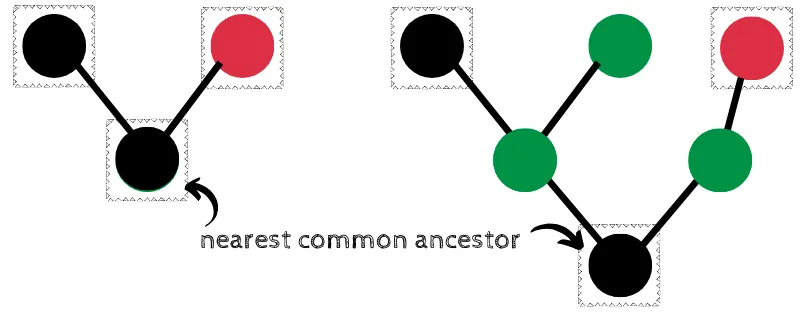
\includegraphics[scale=1]{images/tree_expl_4}
\end{center}
\end{frame}

\section{Methodology}

\section{Results}

\section{Wrap-Up}

{
    \usebackgroundtemplate{\begin{picture}(200,265)
      \includegraphics[width=\paperwidth]{images/beaver_felling_tree}
    \end{picture}}
    \setbeamertemplate{navigation symbols}{}
    \begin{frame}[plain]
    \end{frame}
}

\end{document}